\section{Introduction}
\label{sec:introduction}

Wavetable oscillators store one period and wrap the read pointer at the end of the table.
When those endpoints disagree, each wrap injects a discontinuity that listeners hear as a period-locked click.

\paragraph{Wavetable synthesis in brief.}
A wavetable synthesizer stores a single cycle of a waveform (the wavetable) and produces continuous tone by looping a read pointer through that table.
Pitch is set by how fast the pointer advances. Timbre comes from the stored shape (and, in multi-table banks, from morphing across tables).
Tiling the stored period yields a sustained note under playback.
If the endpoints disagree ($x[0]\neq x[L-1]$), every wrap is a discontinuity at the wrap join (the seam), heard as a click locked to the fundamental.
Figure~\ref{fig:wavetable-primer} shows one stored period, tiled playback with wrap marks, and a zoomed mismatched wrap.
The same geometry appears whenever a short loop is tiled for listening or scoring.

\begin{figure}[t]
  \centering
  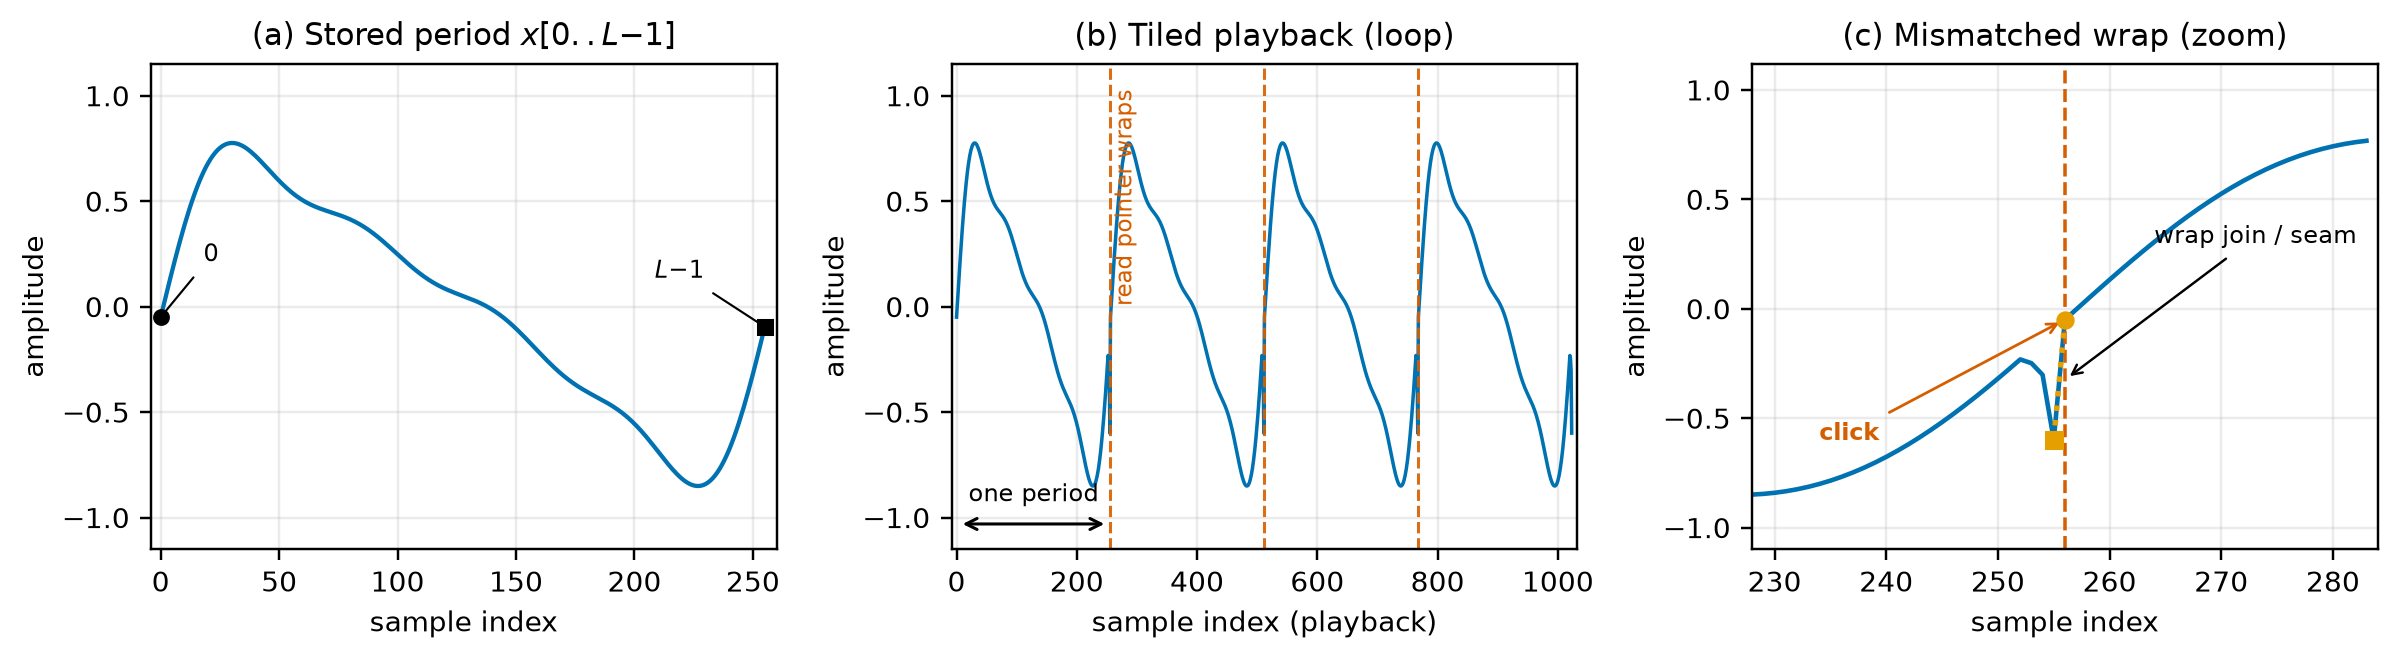
\includegraphics[width=\linewidth]{figures/fig_wavetable_primer.png}
  \caption{Wavetable synthesis primer.
  (a)~One stored period $x[0..L{-}1]$ ($L{=}256$).
  (b)~The same period tiled for continuous playback. Dashed lines mark read-pointer wraps.
  (c)~Zoom at a mismatched wrap join (seam), where the endpoint cliff produces an audible click.}
  \label{fig:wavetable-primer}
\end{figure}

\paragraph{Terminology.}
Key names used below.
A \textbf{seam} (wrap join) is the local end/start junction where endpoint mismatch produces the period-locked click: the seam is local, while the signal is the whole waveform.
\textbf{Repair operator} $\Theta$ means a searchable local edit at that seam (legacy: bake cell), and a tiny network inside $\Theta$ is a \textbf{residual operator}.
\textbf{FitCell} continuously fits one candidate $\Theta$ under residual loss (Appendix~\ref{app:algorithms}).
Scores $R$ and $R_{\mathrm{blend}}$ are unsupervised: prolonged $R$ is debug-only, and $R_{\mathrm{blend}}$ drives primary selection together with the latency-aware objective $J=R_{\mathrm{blend}}-\lambda\cdot\mathrm{latency\_norm}$ (Section~\ref{sec:residual-score}).
\textbf{MoE} soft-gates bake experts, and \textbf{PBT} mutates elites in the outer loop.
The \textbf{outer loop} (meta-search) runs GA plus PPO over repair-operator graphs rather than end-to-end training of one large network.
A \textbf{holdout} freezes the evaluation set or seed for reported scores.

\paragraph{Unsupervised, as used here.}
Search never trains on paired studio-clean audio.
The ideal sibling $r^{\star}$ is a procedural cliff-withheld twin of the cracked engine (self-supervised geometry for scoring), not a human-labeled clean recording.
Operators are ranked under $R_{\mathrm{blend}}$ without requiring labeled clean targets at search time.

We treat the task as \emph{cycle-local seam restoration}: edit a neighborhood of the wrap join (the seam), and optionally a small residual operator over the period, so multi-period playback matches an ideal reference that never opens the wrap cliff.
Agreement uses a discontinuity-weighted blend $R_{\mathrm{blend}}$ (seam fidelity vs the ideal, plus mid-cycle identity vs the cracked engine) under a latency-aware objective $J$ (Section~\ref{sec:residual-score}).

\paragraph{Four roles.}
Keep these distinct (Figure~\ref{fig:intro-sine} and Section~\ref{sec:four-roles}):
\begin{enumerate}
  \item \textbf{Ideal sibling} $r^{\star}$: cliff withheld. Scoring target only. Not a method.
  \item \textbf{No-bake}: unrepaired cracked engine $x$, scored vs $r^{\star}$. A do-nothing reference.
  \item \textbf{Dual Cosine}: classical raised-cosine end fade. Classical baseline.
  \item \textbf{Ours (DenoiseOpt)}: searched repair operator from the hybrid outer loop.
\end{enumerate}
Corrupt-to-corrupt \textbf{Noise2Noise} is a fifth comparator: the primary neural gate under the locked $R_{\mathrm{blend}}$ protocol (Section~\ref{sec:n2n-vs-ours-boards}).
It is not shown in Figure~\ref{fig:intro-sine}, which illustrates roles on one hard sine-wrap tile.

\begin{figure*}[t]
  \centering
  
\includegraphics[width=\textwidth]{figures/fig_intro_sine_problem.png}
  \caption{Hard sine-wrap holdout tile (seed~\texttt{20260719}).
  (a)~Ideal sibling $r^{\star}$.
  (b)~No-bake cracked engine.
  (c)~Dual Cosine fade.
  (d)~Ours (searched bake).
  (e)--(f)~Residual and seam zoom.
  Accompanying JSON scores use locked $R_{\mathrm{blend}}$ ($\alpha{=}0.7$; tile~46: no-bake $0.897$, Dual Cosine $0.300$, Ours $0.989$; Table~\ref{tab:n2n-vs-ours}).}
  \label{fig:intro-sine}
\end{figure*}

Classical virtual-analog tools already address wrap energy locally
(BLIT/BLEP~\cite{stilson1996}, PolyBLEP~\cite{nam2009polyblep}, BLAMP~\cite{esqueda2016blamp}).
We score cycle-local bake versions of those operators beside Dual Cosine (Section~\ref{sec:va-seam-baselines}).
Label-free restoration such as Noise2Noise shows that useful reconstructors can be ranked without paired clean targets when the evaluation geometry is explicit~\cite{lehtinen2018,kashyap2021n2n}.
On the search side, neural architecture search (NAS), aging evolution, PBT, covariance matrix adaptation evolution strategy (CMA-ES), and evolution-guided policy gradients motivate a hybrid outer loop: GA for diversity, PPO for discrete architecture edits, and PBT-style exploit--mutate on elites~\cite{elsken2019,real2019,jaderberg2017,schulman2017,khadka2018}.

\paragraph{Key findings.}
Under the locked v10.1 $R_{\mathrm{blend}}$ protocol with multi-seed evaluation (primary story: Table~\ref{tab:n2n-vs-ours}):
\begin{itemize}
  \item On the primary holdout, the short-FitCell hybrid champion sits just below frozen Noise2Noise---the strongest neural baseline for this locked protocol---on every seed ($0.9708{\pm}0.0014$ vs $0.9767{\pm}0.0015$) and well above Dual Cosine ($0.542{\pm}0.038$).
  \item On twenty multi-family boards, Ours and Noise2Noise are statistically indistinguishable on board-mean deltas ($0.9337{\pm}0.0028$ vs $0.9308{\pm}0.0045$; mean win fraction $0.47$; sign-test $p{=}1.0$).
  \item Matched-$5$k outer-loop comparison ranks hybrid first among six search families ($0.9748{\pm}0.0018$, three search seeds); a hybrid-only FitCell-to-convergence follow-up then clears the Noise2Noise gate on the \emph{single completed} search seed \texttt{1902771841} ($R_{\mathrm{blend}}{\approx}0.9912$; Section~\ref{sec:v14-converge}).
  \item On hard wrap cliffs, classical fades collapse while searched operators and Noise2Noise hold (Section~\ref{sec:cliff-strata}).
  \item On Factory+FX and AKWF corpora under $R_{\mathrm{blend}}$, Noise2Noise leads Ours; both still beat Dual Cosine.
\end{itemize}
We do not claim a new NAS/RL algorithm.
Existing NAS, aging evolution, PBT, CMA-ES, and PPO primitives are reused~\cite{elsken2019,real2019,jaderberg2017,schulman2017}.
The contribution is applying a hybrid GA+PPO(+PBT) outer loop to \emph{compact cycle-local repair operators} for wavetable wrap discontinuity under an unsupervised sibling score, then selecting hybrid from a matched six-way bake-off before deepening FitCell.
Compact searchable repair operators remain competitive when classical fades fail and need no paired clean targets at search time.
Whole-curve prolonged $R$ near $0.991$ is a superseded debug score, not a current holdout result under $R_{\mathrm{blend}}$.

\paragraph{Transfer datasets.}
Transfer boards apply the \emph{same} wrap-discontinuity protocol to other short periodic signals
(Section~\ref{sec:transfer-protocol}): open a cliff at the period join, score against a no-cliff ideal sibling.
They are mechanistic stress tests of wrap geometry under that protocol, not evidence of general domain diagnosis.
Boards: \textbf{CWRU}, \textbf{MFPT}, and \textbf{Paderborn} K001 (one shaft revolution as a period),
\textbf{MIT-BIH} and a \textbf{PTB-XL} 500\,Hz subset (one heartbeat as a period),
plus \textbf{synthetic CNC} and \textbf{synthetic PMU/AC} pilots when real downloads are walled
(Table~\ref{tab:transfer-main}).

\paragraph{Scope.}
Cycle-local wavetable seam repair for DSP / synthesis venues (DAFx / AES / arXiv cs.SD).
Formal wrap-closure proofs, search-convergence theorems, and speech/music enhancement SOTA are out of scope; caveats live in Section~\ref{sec:limitations}.

\subsection{Contributions}
\label{sec:contributions}
\begin{enumerate}
  \item \textbf{Problem framing.} Wrap discontinuity as cycle-local seam restoration under tiled evaluation, with explicit $R_{\mathrm{seam}}$, $R_{\mathrm{body}}$, and primary locked $R_{\mathrm{blend}}$ ($\alpha{=}0.7$) plus latency-aware $J$.
  \item \textbf{Ideal-sibling protocol.} Unsupervised scoring via a procedural cliff-withheld twin plus mid-cycle engine identity, without paired studio-clean targets at search time.
  \item \textbf{Compact repair-operator space.} Searchable graphs over classical seam ops (DualCosine, FIR, VA residuals) and tiny residual nets (MLP/FIR/U-Net-lite/LSTM-lite/MoE), not end-to-end Demucs-scale stacks (Section~\ref{sec:bake}, Appendix~\ref{app:algorithms}).
  \item \textbf{Applied hybrid search + selection evidence.} DenoiseOpt applies GA--PPO(+PBT) to that operator space; a matched six-way $5$k bake-off under locked $R_{\mathrm{blend}}{+}J$ ranks hybrid first, motivating hybrid-only FitCell-to-plateau (Tables~\ref{tab:meta-approaches},~\ref{tab:v14-hybrid-converge}).
  \item \textbf{Open multi-seed evaluation.} Frozen Noise2Noise gate, five-seed holdout, multi-family and wavetable-native boards, hard-cliff strata, wrap-protocol transfer stress tests, and released code/artifacts (\texttt{REPRO.md}).
\end{enumerate}
What is \emph{not} claimed as a contribution: a new foundational NAS/RL algorithm, formal wrap-closure theorems, or perceptual MOS/MUSHRA superiority.
